\documentclass{beamer}

\usepackage{beamerthemesplit}
\usepackage{verbatim}

\usetheme{Pittsburgh}
%\usecolortheme{seagull}
%\usecolortheme{seahorse}
\usecolortheme{beaver}

\usefonttheme{serif}

%\DeclareGraphicsExtensions{.pdf,.png,.jpg}

\newcommand{\snT}{$(S/N)_{\textrm{size}}$}
%\newcommand{\snT}{$\left( \frac{S}{N}\right)_{\textrm{size}}$}
\newcommand{\snflux}{$(S/N)_{\textrm{flux}}$}
%\newcommand{\snflux}{$\left( \frac{S}{N}\right)_{\textrm{flux}}$}

\newcommand{\lensfit}{\texttt{LENSFIT}}
\newcommand{\numba}{\texttt{Numba}}
\newcommand{\python}{\texttt{Python}}
\newcommand{\ngmix}{\texttt{ngmix}}
\newcommand{\shear}{{\bf g}}
\newcommand{\redmapper}{redMaPPer}

\newcommand{\prelim}{{\bf{\it Preliminary}}}

\title{Weak Lensing Results from DES}
\author{Erin Sheldon, and the DES Lensing Working Group}
\institute{Brookhaven National Laboratory}

% http://texblog.net/latex-archive/plaintex/beamer-footline-frame-number/
% to add the page (frame ) number and not screw up the bottom line
% works for split themes?
\expandafter\def\expandafter\insertshorttitle\expandafter{%
      \insertshorttitle\hfill%
        \insertframenumber\,/\,\inserttotalframenumber}

% suppress navigation bar
\beamertemplatenavigationsymbolsempty

\begin{document}

\frame{\titlepage}

%\section{Dark Energy}

\frame
{
    \frametitle{Outline}

    \begin{itemize}

        \item Introduction to Dark Energy and Lensing

        \item The Dark Energy Survey

        \item \prelim\ Lensing Results for Galaxy Clusters

    \end{itemize}


}


\frame
{
    \frametitle{Dark Energy}

    \fontsize{9}{0.8\baselineskip}
    \begin{columns}
        \begin{column}{0.5\textwidth}    
            \begin{itemize}

                \item The original story is simple: there are objects whose
                    intrinsic brightness we think we know (type 1a supernovae)

                \item If we know one of these objects is at a given redshift we
                    should be able to predict its observed brightness: $D(z)$.

                \item It turns out this only works if we modify the equations
                    so that the universe is accelerating at late times
                    %(long
                    %after the big bang, recently) instead of slowing down

                %\item modifies the relation between the observable redshift $z$
                %    and distance.

                \item Either add a new component, such as a cosmological constant,
                    or modify general relativity

            \end{itemize}
        \end{column}
        \begin{column}{0.5\textwidth}
            \begin{center}
                \includegraphics[width=\textwidth]{riess-distmodulus.pdf}
                \newline
                Riess et al. 2007
            \end{center}
        \end{column}
    \end{columns}
}

\frame
{
    \frametitle{Standard Rulers}

    \fontsize{9}{0.8\baselineskip}
    \begin{columns}
        \begin{column}{0.5\textwidth}    
            \begin{itemize}

                \item The baryon acoustic feature is frozen in when the
                    universe cools enough for baryons and photons to decouple:
                    it is thus a standard ruler

                \item Its apparent size at a given redshift should be predictable
                    given the observed size in the CMB and a cosmological model $D(z)$.

                \item Again, it only works if we modify the equations.

                \item Agreement with supernovae

            \end{itemize}
        \end{column}
        \begin{column}{0.5\textwidth}
            \begin{center}
                \includegraphics[width=\textwidth]{bao-all.pdf}
                \newline
                Aubourg et al. 2014 (BOSS)
            \end{center}
        \end{column}
    \end{columns}
}

\frame
{
    \frametitle{Simplest Possible Components}

    \begin{itemize}

        \item Add a constant energy density component to the stress-energy:   A
            cosmological constant $\Lambda$ that has equation of
            state  $p=-\rho$.
            
        \item Constant energy density in an expanding universe is unsatisfying,
            but it matches the data well with our current limited precision.

        \item Next level of complexity: arbitrary equation of
            state\footnote{Any accelerating solution for $w$ ($< - 1/3$)
            violates the strong energy condition.}.  This is poorly constrained
            with current data.

    \end{itemize}

    \begin{equation}
        p = w \rho
    \end{equation}

    %\begin{itemize}
    %    \item Any accelerating solution $w$ ($< - 1/3$) violates the strong energy condition.
    %\end{itemize}

}



\frame
{
    \frametitle{Gravitational Lensing}

    \begin{itemize}

        \item Light is deflected as it passes massive bodies.

        \item All objects in the universe are lensed.

        \item As with an ordinary lens, the deflection at the detector depends
            on the strength of the lens and the geometry of the
            lens-source-observer system

        \item The geometry depends on dark energy.
            
        \begin{itemize}
            \item We can use this to measure dark matter and dark energy
        \end{itemize}

    \end{itemize}

}

\frame
{
    \frametitle{Lensing Geometry}

    \includegraphics[width=\textwidth]{lens_geometry.pdf}

}

\frame
{
    \frametitle{Example: Lensing Geometry and Dark Energy}

    %\fontsize{9}{0.8\baselineskip}
    \begin{columns}
        \begin{column}{0.5\textwidth}    
            \begin{itemize}

                \item The signal depends on the distance of source behind
                    the lens.


                \item Measure the lensing effect using the same lens and sources
                    at different distances

                \item the mapping beteween distance and observables (redshift) 
                    depends on dark energy

                \item What value of the equation of state $w$ do we need to
                    describe the observations?

            \end{itemize}
        \end{column}
        \begin{column}{0.5\textwidth}
            \includegraphics[width=\textwidth]{scinv-example.pdf}
        \end{column}
    \end{columns}
}


\frame
{
    \frametitle{Lensing Reality}

    \begin{center}
        \includegraphics[width=\textwidth]{shear-illustration.jpg}
        \newline
    \end{center}

}


\frame
{

    \frametitle{Weak Lensing}

    \fontsize{10}{0.8\baselineskip}

    \begin{columns}

        \begin{column}{0.5\textwidth}

            \begin{itemize}

                \item We don't see the deflection directly.

                \item The ``deflection'' can differ across the face of an
                    extended source galaxy, causing distortion.

                \item We say the image is ``sheared'' (a light bundle 
                    is sheared)

                \item For small shears, a circle becomes a pure ellipse.

                \item Shearing produces correlations in the shapes of galaxies across the sky.
                    Shape correlations are closely related to mass density
                    correlations.

            \end{itemize}
        \end{column}
        \begin{column}{0.5\textwidth}
            \includegraphics[width=\textwidth]{shear-illustration-crop.jpg}
            \newline
            \begin{center}
                {\small Note galaxies aren't round!  ``Shape noise''}
            \end{center}
        \end{column}
    \end{columns}
}


\frame
{

    \frametitle{Weak Lensing}

    \fontsize{10}{0.8\baselineskip}

    \begin{columns}

        \begin{column}{0.5\textwidth}

            \begin{itemize}

                \item The ``tangential'' stretching seen here is indicative
                of a generic symmetry

                \item When averaged over a large sample, there are no ``B-modes'',
                    only ``E-modes''

                \item Later I will discuss shear correlation measurements for both modes.

            \end{itemize}
        \end{column}
        \begin{column}{0.5\textwidth}
            \begin{center}
                \includegraphics[width=0.7\textwidth]{shear-illustration-crop.jpg}
                \newline
                \includegraphics[width=0.7\textwidth]{EBmode.pdf}
                \newline
                {\tiny Baumann http://arxiv.org/abs/0907.5424}
            \end{center}
        \end{column}
    \end{columns}
}



\frame
{
    \frametitle{Shear}
    %\fontsize{10}{0.8\baselineskip}

    \begin{columns}
        \begin{column}{0.5\textwidth}
            \begin{itemize}


                \item The correlations in the shear/matter field hold a lot of
                    information about the {\bf Dark Matter} distribution.  The Cold Dark
                    Matter theory predicts these correlations.

                \item Shear depends on the distances to the lens and source. The
                    distance dependence encodes the expansion rate of the universe and
                    thus {\bf Dark Energy}.

                %\item To meet goals of current surveys we want to measure shear to
                %    about 0.4\% accuracy (e.g.  Dark Energy Survey).  LSST about
                %    a factor of five better.

            \end{itemize}
        \end{column}

        \begin{column}{0.5\textwidth}
                \includegraphics[width=\textwidth]{berlind-weinberg-f3.pdf}
                \newline
                Berlind \& Weinberg 2002
                \newline
                Dark Matter Prediction
        \end{column}
    \end{columns}
}


\begin{comment}
\frame
{
    \frametitle{Lensing Dark Energy State of the Art}

    \begin{center}
        \includegraphics[width=\textwidth]{cfht-wmap.pdf}
        \newline
        Kitching et al. 2015, CFHTLens.  Pure ``Cosmic Shear'' measurement.
    \end{center}

}
\end{comment}



\frame
{
    \frametitle{Shear From Galaxy Clusters}

    \begin{center}
        \includegraphics[width=0.8\textwidth]{maxbcg_sample21-22_ngals200_12_jackknife.pdf}
        \newline
        Sheldon et al. 2009.  MaxBCG Clusters from the Sloan Digital Sky Survey Galaxy Clusters
    \end{center}
}



\frame
{
    \frametitle{Galaxy Clusters in the SDSS}
    \fontsize{10}{0.8\baselineskip}

    \begin{columns}
        \begin{column}{0.5\textwidth}
            \begin{itemize}

                \item This technique is well established, and measurements have high precision.

                \item In SDSS we used lensing to study the dark matter distribution in
                    and around galaxy clusters.

                \item SDSS is a low redshift survey, no sensitivity to dark energy.

                \item Similar measurements by other surveys (e.g. CFHT, Weighing the Giants)
                    as well as more generic shear measurements (``Cosmic Shear'')

            \end{itemize}
        \end{column}

        \begin{column}{0.5\textwidth}
            \begin{center}
                \includegraphics[width=\textwidth]{maxbcg_sample21-22_ngals200_12_jackknife.pdf}
                \newline
                Sheldon et al. 2009
            \end{center}
        \end{column}
    \end{columns}
}


\frame
{
    \frametitle{Dark Energy Survey (DES)}

    \fontsize{9}{0.8\baselineskip}
    \begin{columns}
        \begin{column}{0.5\textwidth}    
            \begin{itemize}

                \item Imaging survey of 5000 square degrees in the 
                    southern sky (CTIO) through 5 optical filters.  Depth $\sim 24$ in
                    $i$-band.

                \item Study dark energy using weak lensing, galaxy clusters, supernovae
                    and large scale structure (BAO).

                \item First light fall 2012, survey start Aug. 31 2013
                    
                \item Can repeat SDSS cluster measurements with equal S/N at
                    many redshifts: Dark Energy

                \item Next generation:  reduce the errors on $w$ to the percent level.

            \end{itemize}
        \end{column}
        \begin{column}{0.5\textwidth}
            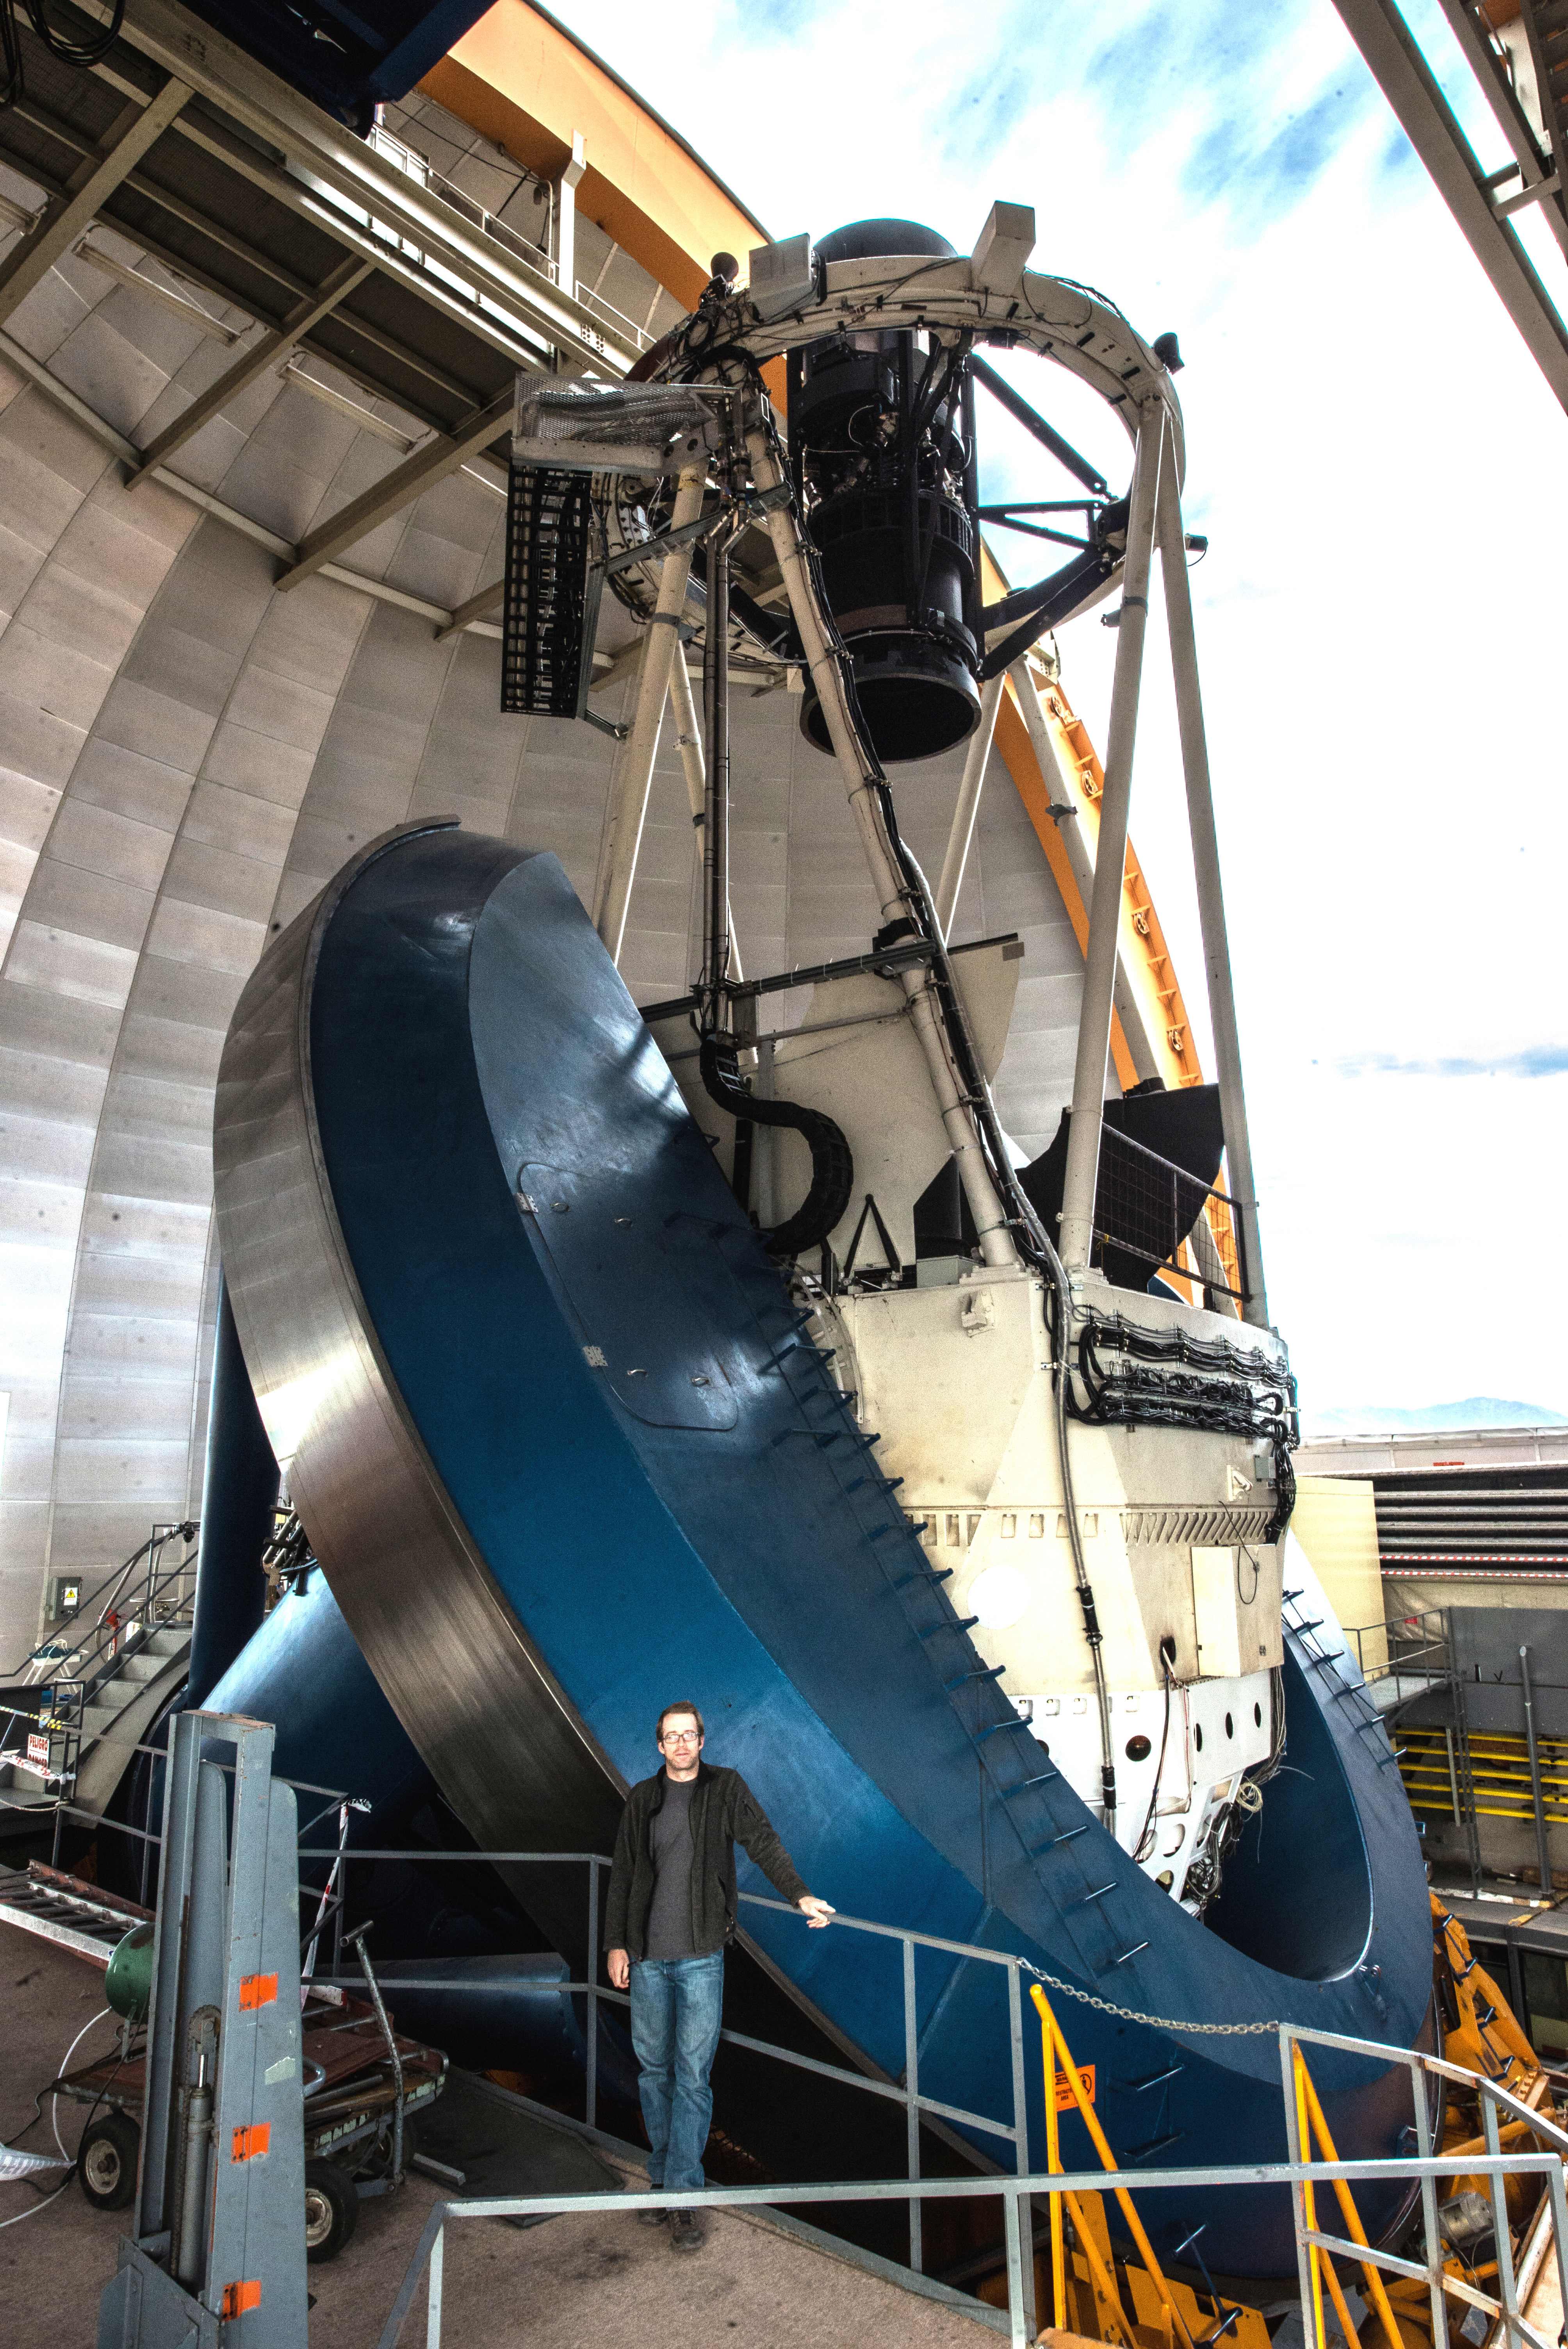
\includegraphics[width=\textwidth]{ctio_blanco_crew_2013Oct-19-contrast.jpg}
        \end{column}
    \end{columns}
}


\frame
{
    \frametitle{What is needed to achieve DES goals}

    %\fontsize{9}{0.8\baselineskip}
    \begin{itemize}

        \item Measure the shears with $\sim$ 0.4\% accuracy (1-2\% for early data).

            \begin{itemize}
                \item Develop galaxy shape measurement algorithms
            \end{itemize}

        \item Measure the distances with equal accuracy.

        \begin{itemize}
            \item No spectra, so this means photometric redshifts.
        \end{itemize}

    \end{itemize}
}

\frame
{
    \frametitle{Measuring Shear}

    \begin{itemize}

        \item For a perfect detector with no noise, just measure
            the second moments and look for the correlations.

        \item ... but the atmosphere, telescope, and instrument smear
            the image: the Point Spread Function (PSF).

        \item Convolution just adds to the moments, so we just need to
            subtract off the PSF moments!

        \item ... but there is noise, so error in moments blows up (among other
            difficulties).

    \end{itemize}

    \begin{center}
        \includegraphics[width=0.8\textwidth]{great3-systematics.pdf}
        \newline
        GREAT3 Team
    \end{center}

}

\frame
{
    \frametitle{DES Shear Measurement Codes}

    %\fontsize{9}{0.8\baselineskip}
    \begin{itemize}

        \item In DES we have three shear measurement methods, all of which
            overcome the above difficulties

        \item For all methods we fit an elliptical model, such as an elliptical
            exponential disk, to galaxies.  We use the ellipse parameters as
            measurements of the shear

        \begin{itemize}
            \item LENSFIT style method, based on Miller et al. 2007

            \item Bayesian shear estimation based on Bernstein \& Armstrong 2014

            \item im3shape measurement, Zuntz et al. 2013
        \end{itemize}

        \item In this talk I will focus on my implementations of
            LENSFIT and B\&A

    \end{itemize}
}

\frame
{
    \frametitle{Common Features of All Methods}

    \begin{itemize}
        
        \item The Point Spread function of the telescope and atmosphere blurs
            out the images.  We must determine this from stars and correct for it.
            We use PSFEx. (Bertin)
        
        \item There are small distortions in the optics (not convolutions).
            These must be mapped and included in the analysis.
            We use SCAMP. (Bertin)

        \item Fit a model to each galaxy, convolved with the interpolated PSF
            and estimated in the {\it undistorted} frame.

        \item ``multi-fit'': We have of order 10 epochs.  Rather than use the coadd image
            we do the fit using all the epochs simultaneously.  This avoids
            discontinuities in the PSF.

        \item Mitigate noise-related calibration biases

    \end{itemize}
}

\frame
{
    \frametitle{How Can We Test Shear Methods?}

    \begin{itemize}

        \item No absolute calibration source for shear: we need to use
            simulations to test overall calibration

        \item Null tests (not exhaustive)

            \begin{itemize}

                \item In the absence of systematics, the mean shear should be
                    zero over a large enough area of sky

                \item The shear should not correlate with star shapes if we
                    corrected properly for the PSF.

                \item The shear should have the correct symmetries.  There
                    should be no curl-like ``B-mode'' patterns.

            \end{itemize}

    \end{itemize}
}

\frame
{
    \frametitle{Bayesian Shear Measurement: Bernstein \& Armstrong 2014}

    \begin{itemize}

        \item Shape of a noisy galaxy is a biased estimate of shear

        \item Forget about shear from a single galaxy image.

        %\item While the posterior surface for the {\it shape} of single galaxy
        %    is complex, the posterior surface for the {\it mean shear} of an
        %    ensemble must approach a Gaussian according to the central limit
        %    theorem.  This is both useful and actually true!

         \item Assuming weak shear, and knowledge of underlying distribution of
             shapes for the ensemble (the prior), one can derive an unbiased
             estimator for the mean shear of the {\it ensemble}.

         \item You lose nothing: in the limit of weak shear, you need
             to use an ensemble statistic anyway.  The ``shape noise'',
             intrinsic variance in shapes of galaxies, dominates over
             the signal.

        \item I developed an implementation, presented in Sheldon 2014
         
    \end{itemize}

}


\frame
{
    \frametitle{Bayesian Lensing Shear Measurement: \ngmix}

    \fontsize{9}{0.8\baselineskip}
    \begin{columns}
        \begin{column}{0.4\textwidth}
            \begin{itemize}

                \item Figure: Fractional error in the shear
                    %for simulated galaxies
                    %(exp,dev profiles) near smallest usable {\it observed} size
                    %fwhm/fwhm$_{\textrm{psf}}$ = 1.2.

                \item Light grey: DES requirements, dark grey: LSST requirements

                \item Current limitations:  very small shear ($\sim 0.01$) and 
                    constant shear only.

                \item We think we will ultimately use this method, but shelved
                    for now until we address limitations (See Madhavacheril et
                    al.)

            \end{itemize}
        \end{column}
        \begin{column}{0.6\textwidth}
            \begin{center}
                \includegraphics[width=\textwidth]{ngmix-flux-s2n-sigrat-20.pdf}
                \newline
                Sheldon 2014
            \end{center}
        \end{column}
    \end{columns}

}



\frame
{
    \frametitle{LENSFIT implementation: \ngmix}

    \begin{itemize}

        \item Use priors on the parameters and explore a constrained posterior
            surface (Prior $\times$ Likelihood).

        \item Derive approximately how the shear estimate (the shape) responds
            to a small shear in the presence of the noise and prior.
            
        \item This {\bf response} is calculated using integrals over the
            posterior surface and first order approximation in shear.

        %\item The posterior surface of the shape for a single galaxy is
        %    complex.  The space is bounded, the surface is necessarily
        %    asymmetric and depends on galaxy properties and noise.

        \item No rigorous expression is given for the mean shear of a
            population given these responses.  Choose to simply average them.
        
    \end{itemize}
}


\frame
{
    \frametitle{\ngmix\ Tests with simulations}

    \fontsize{9}{0.8\baselineskip}
    \begin{columns}
        \begin{column}{0.3\textwidth}
            \begin{itemize}

                %\item Top Figure: Fractional error in the shear for simulated galaxies
                %    (exp,dev profiles) 

                %\item Bottom Figure: Fractional error in the shear using real galaxy
                %    images from COSMOS, sheared, convolved and noised.
                \item Fractional error in the shear using real galaxy
                    images from COSMOS, sheared, convolved and noised.

                \item Works well at high shear.

                \item Good enough for early DES data.

            \end{itemize}
        \end{column}
        \begin{column}{0.7\textwidth}
            \begin{center}
                \includegraphics[width=\textwidth]{noise-bias-ngmix.png}
                \newline
                Kacprzak, T.
            \end{center}
        \end{column}
    \end{columns}

}


\frame
{
    \frametitle{\ngmix\ Null Tests on DES Data: B modes}

    \begin{itemize}

        \item If the shear we measure is due to lensing, it must have
            certain symmetries: No B-modes allowed

        \item Error bars from simulations
        
        \item Consistent with zero

    \end{itemize}

    \begin{center}
        \includegraphics[width=0.8\textwidth]{ngmix009_b.pdf}
        \newline
        Matthew Becker (Stanford/SLAC)
    \end{center}

}


\frame
{
    \frametitle{\ngmix\ Null Tests on DES Data: PSF Leakage}

    \begin{itemize}

        \item If our PSF correction is working, there should be no relation between
            measured galaxy shape and PSF shape.

        \item DECam PSF are quite round 

        \item The relation is weak but detected.

    \end{itemize}


    \begin{center}
        \includegraphics[width=0.8\textwidth]{ngmix011-e-vs-epsf-Ts2n-min-300-s2n-min-10.pdf}
    \end{center}

}


\frame
{
    \frametitle{\ngmix\ Null Tests on DES Data: Galaxy Size}

    \begin{itemize}

        \item The mean shape should not depend on the galaxy size.

        \item The absolute values are not huge (0.5\%) but clearly detected.
        
        \item Seems to mostly average out over the whole sample

    \end{itemize}


    \begin{center}
        \includegraphics[width=0.5\textwidth]{ngmix011-e-vs-sigma-mx-50-Ts2n-min-300-s2n-min-10.pdf}
    \end{center}

}



\frame
{
    \frametitle{\prelim\ Results: Lensing with \redmapper\ Clusters}
    
    \begin{itemize}

        \item Select large contiguous area from DES Early Data: $\sim 162$ square degrees
            in the SPT region.

        \item Select galaxy clusters using the \redmapper\ algorithm (Rykoff,
            Rozo et al. 2014).  $\sim$ 12,000 groups and clusters with redshift
            $z \in [0.2,0,0]$

        \item Measure the ensemble lensing signal around sets of clusters.

        \item Repeat SDSS analysis: Bin cluster by ``richness', look for mass scaling.

    \end{itemize}
}

\frame
{
    \frametitle{DES Region ``SPT-E''}

    \begin{itemize}

        \item $\sim 162$ square degrees

        \item Full survey depth: 10 epochs, $i$-band 10-$\sigma$ limiting magnitude
            $\sim$ 24

    \end{itemize}

    \begin{center}
        \includegraphics[width=0.8\textwidth]{spte-greyscale-density-010000000.pdf}
    \end{center}

}

\frame
{
    \frametitle{\prelim\ Results: Lensing with \redmapper\ Clusters}

    \begin{itemize}

        \item Overall mean shear signal for 12,000 clusters

        \item No corrections at low radius for cluster members or deblending issues

    \end{itemize}

    \begin{center}
        \includegraphics[width=0.6\textwidth]{run-rm008-bin-zwide-jack.pdf}
    \end{center}

}


\frame
{
    \frametitle{\prelim\ Results: Lensing with \redmapper\ Clusters}

    \begin{itemize}

        \item Dependence on richness $\lambda$.

        \item No corrections at low radius for cluster members or deblending issues

    \end{itemize}


    \begin{center}
        \includegraphics[width=0.6\textwidth]{run-rm008-bin-lbin4-zwide-jack.pdf}
    \end{center}

}

\frame
{
    \frametitle{\prelim\ Results: Lensing with \redmapper\ Clusters}

    \begin{itemize}

        \item Dependence on lens redshift.

        \item No corrections at low radius for cluster members or deblending issues

    \end{itemize}


    \begin{center}
        \includegraphics[width=0.6\textwidth]{run-rm008-bin-lgt05-zbin4-jack.pdf}
    \end{center}

}

\frame
{
    \frametitle{Future Work}

    \begin{itemize}

        \item Process more data!

        \item Model the profiles using a simple halo model to extract
            mass and clustering information.

        \item Combine mass-$\lambda$ relation with the abundance of clusters to
            constrain the ``mass function''.

        \item Use the redshift dependence to constrain dark energy.

    \end{itemize}

}

\frame
{
    \frametitle{Summary}

    \begin{itemize}

        \item Lensing is a promising method to constrain Dark Energy

        \item The Dark Energy Survey is underway.  We have significant shear measurements
            with early data.

        \item We have multiple promising shear pipelines, and are passing most
            of our calibration and null tests.


    \end{itemize}

}




\end{document}
